Whereas, people have have often tried to categorized objects as GCs by making
cuts along half-light radius, density, and surface brightness profile, in fact
many objects which are generally thought of as GCs don't cleanly fit into these
cuts. Consequently, \citet{Carretta2010} proposed a definition of GC based on
observed chemical inhomogeneities in their stellar populations. The modern
understanding of GCs then is not simply one of a dense cluster of stars which
may have chemical inhomogeneities and multiple populations; rather, it is one
where those chemical inhomogeneities and multiple populations themselves are
the defining element of a GC.

All globular clusters older than 2 Gyr studied in detail show populations
enriched in He, N, and Na while also being deplete in O and C
\citep{Piotto2015,Bastian2018}. These light element abundance patterns also are
not strongly correlated with variations in heavy element abundances. One
consequence of this fact is the aforementioned spectroscopically uniform Fe
abundances. Further, high-resolution spectral studies reveal anti-correlations
between N-C abundances, Na-O abundances, and potentially Al-Mg
\citep{Sneden1992, Gratton2012}. Typical stellar fusion reactions can deplete
core oxygen; however, the observed abundances of Na, Al, and Mg cannot be
explained by the likes of the CNO cycle \citep{Prantzos2007}.

Formation channels for these multiple populations remain a point of debat
amoung astronomers. All seriously considered formation channels consist of some
older, more massive, population of stars polute the prisine cluter media before
a second population forms, now enriched in heavier elements they themselves
could not have generated [CITE]. The three primary candidates for these
poluters are asymtotic giant branch stars (AGBs), fast rotating massive stars
(FRMSs), and very massive stars (VMSs). Hot hydrogen burning is a feature of
each of these models and consequently they all {\it qualitativley} agree with
the observed elemental abundances. However, non of the standard models can
currently account for all specific abundances [CITE].

Despite these challenges, predictions of He enhancement distinguishing MPs have
lined up well with isochrone fitting results. Therefore, it is currently
accepted that MPs are primarily parameterized by their Helium abundances
[CITE]. Depending on the cluster, Ys as high as 0.4 have been inferred [CITE].
However, due to the relatively high and tight temperature range of partial
ionization for He it cannot be observed in globular clusters; consequently, the
evidence for enhanced He in GCs originates from comparison of theoretical
stellar isochrones to the observed color-magnitude-diagrams of globular
clusters. Therefore, a careful handling of chemistry is essential when modeling
with the aim of discriminating between MPs; yet, only a very limited number of
GCs have yet been studied with chemically self-consistent (structure and
atmosphere) isochrones \citep[e.g.][NGC 6752]{Dotter2015}.

This thesis will contain chapters where we expand the number of clusters which
have been self-consistently modeled. In this chapter we will focus on the two
extreme population of NGC 2808 identified by [CITE], A and E.

\subsubsection{Population Opacities}
For similar reasons as discussed in \S\ref{sec:japGap1} we conduct this research
with OPLIB high-temperature opacity tables as opposed to OPAL tables. We use
our OPLIB web scraper to generate opacity tables with compositions specific to
each population in NGC 2808.

These population have been studied in depth by Feiden and their chemical
compositions were determined in \citet{Milone2015} (see Table 2 in that paper).
While we cannot currently make fully self-consistent models due to still
ongoing atmospheric modeling, we can make a first pass investigation of the
affect of OPLIB opacities (Figure \ref{fig:NGC2808ISO}). Note how the models
generated using OPLIB opacity tables have a systematically lower luminosity.
Recall, that this is consistent with the overall lower opacities of the OPLIB
tables.

\begin{figure}
	\centering
	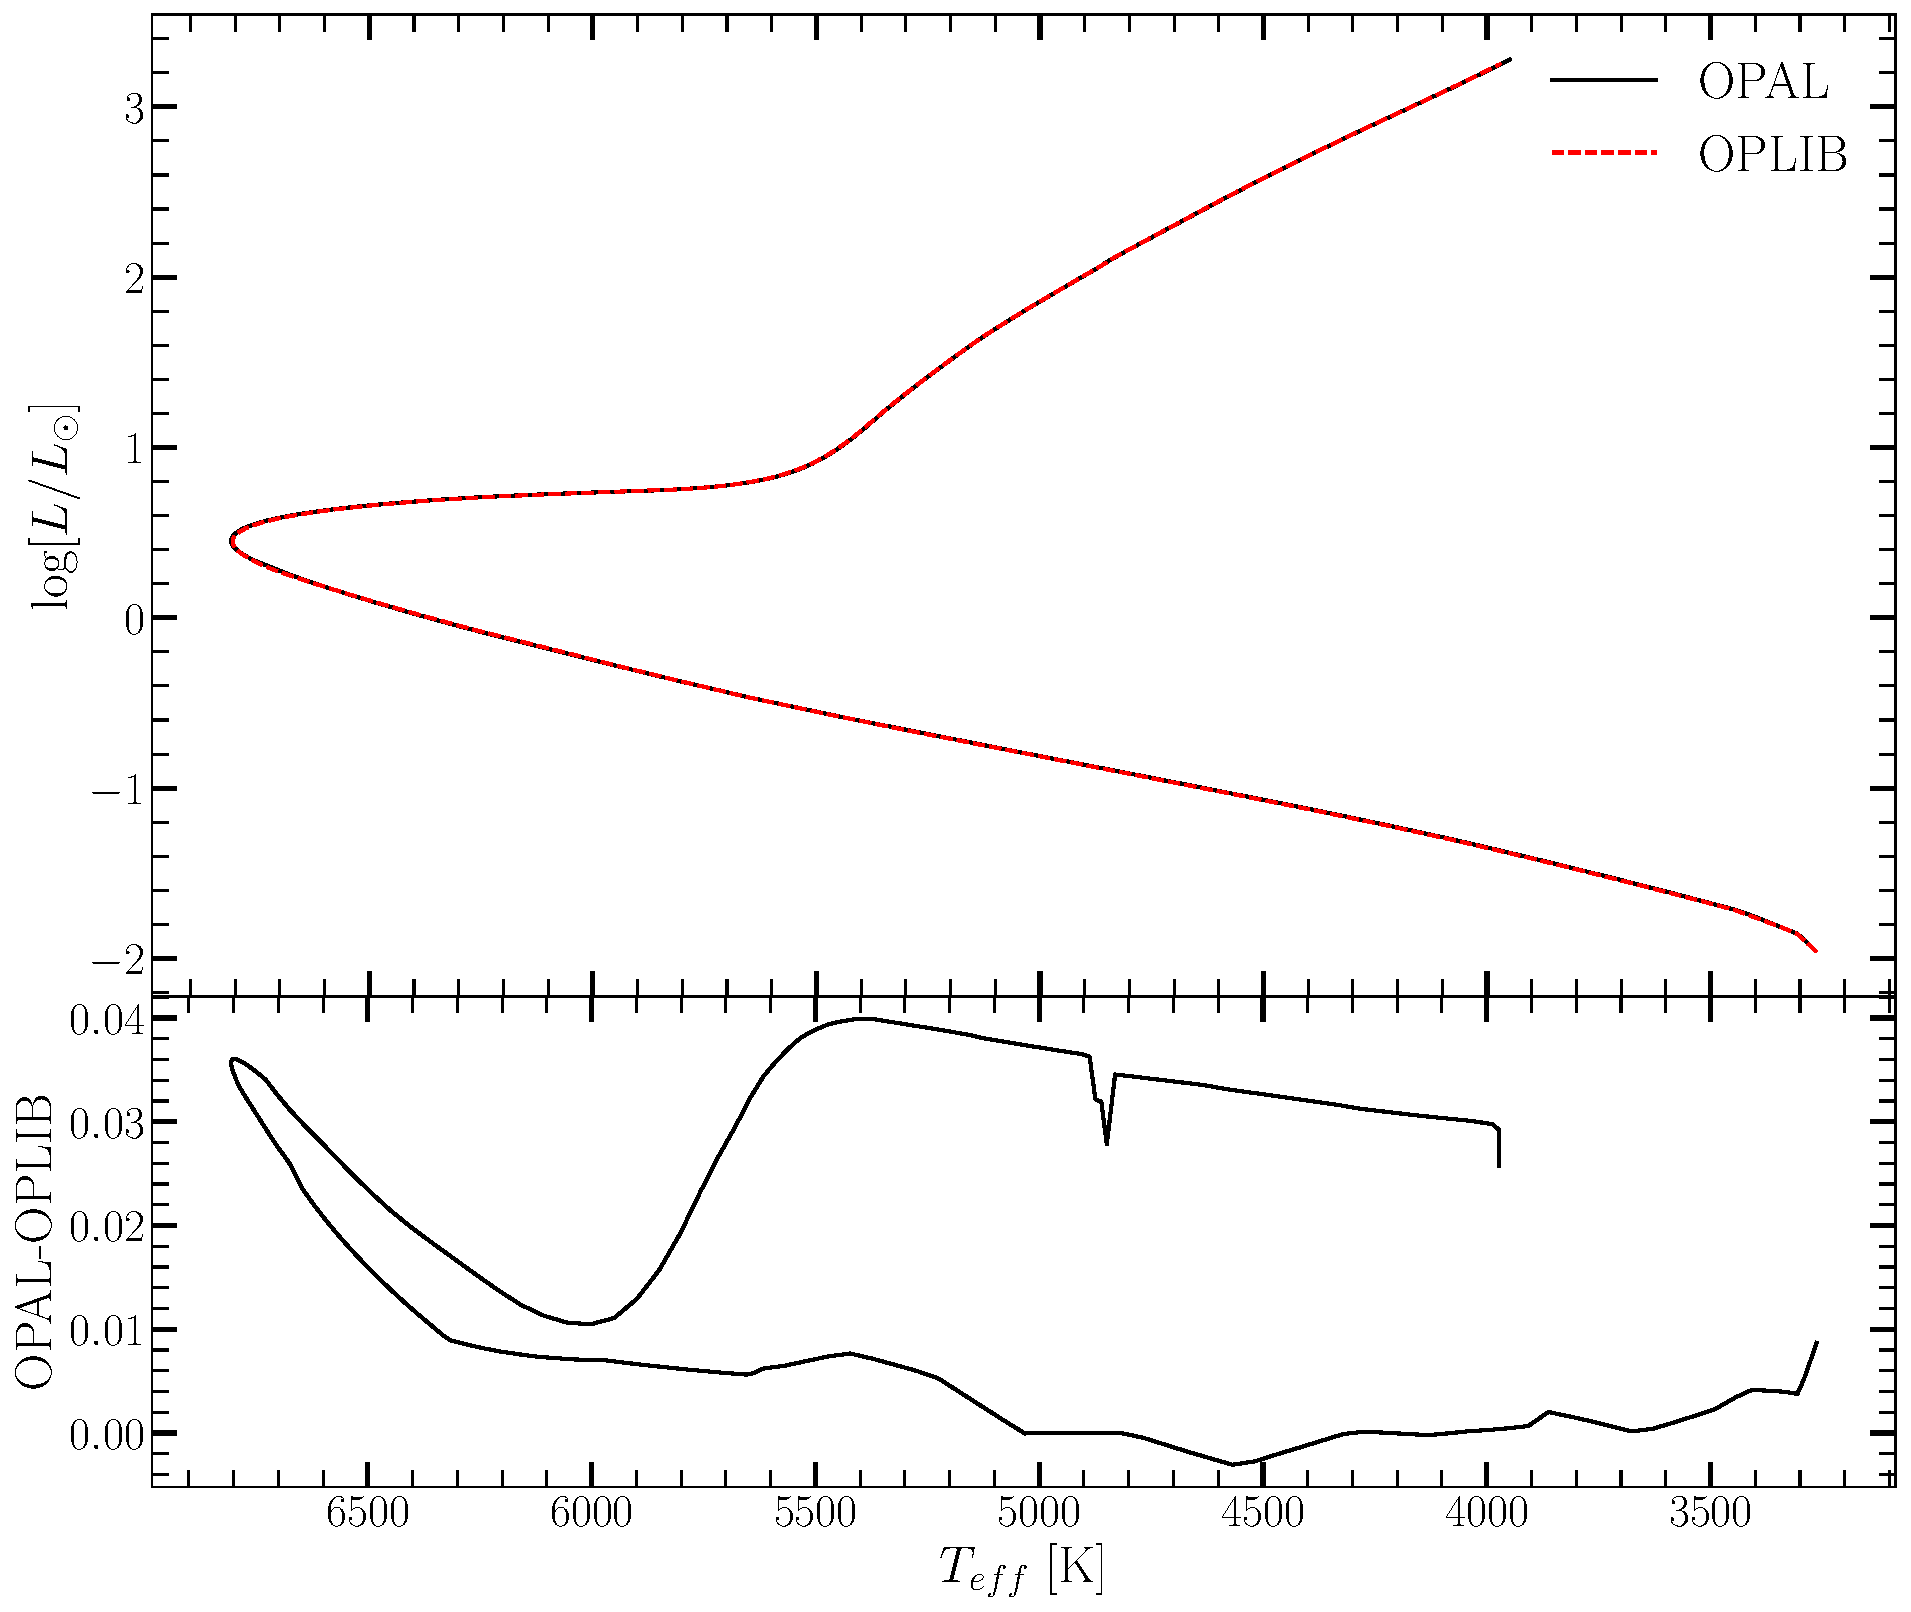
\includegraphics[width=0.45\textwidth]{src/Figures/033ZIsosOPALOPLIB.pdf}
	\caption{10 Gyr \& Y=0.33 isochrones for models generated with OPAL and
	OPLIB opacities tables (top). Residuals between isochrones (bottom).}
	\label{fig:NGC2808ISO}
\end{figure}

\subsubsection{Additional Consistency}
The lack of self consistency presents problems at other stages of stellar
evolution codes. Perhaps most importantly, where the interior of a stellar
model meets the atmosphere. Atmospheric models such as a grey
\citep{Eddington1916}, Krishna Swamy \citep{Krishna1966}, or Phoenix
\citep{Husser2013} model atmosphere provide one pressure boundary conditions to
solve the two-point boundary value problem that is the equations of stellar
structure. Once again however, models tend to use atmospheres with non
consistent chemistries. Therefore, one key element of NGC 2808 modeling is the
incorporation of new atmospheric models, generated from the MARCS grid of model
atmospheres \citep{Plez2008}, which match interior elemental abundances.
Members of our collaboration are currently working on such atmospheric
modeling.

Finally, The isochrones used to infer the degree of helium enhancements assume
that convection operates in the same manner in metal-poor stars as it does in
the Sun. However, observations from \textit{Kepler} of metal-poor red giants
\citep{Bonaca2012, tayar2017correlation}, in concert with interferometric
radius determination of the metal-poor sub-giant HD 140283
\citep{creevey2015benchmark}, have shown that the efficiency of convection
changes with iron content. We will additionally modify DSEP to capture this
variation in convective efficiency. While we wait for atmospheric modeling to
be completed it makes sense to investigate other locations where opacity
differences on the order of 5\% may affect results."s
